\chapter[Pruebas]{
  \label{chp:pruebas}
  PRUEBAS
}
\thispagestyle{numberingStyle}
\pagestyle{numberingStyle}

En este apartado se comentarán las pruebas realizas para verificar el correcto funcionamiento de la aplicación.



\section{Pruebas de integración}
Estas pruebas son realizadas para probar la correcta interacción entre dos o más unidades software. Para que estas pruebas sean de validez, es necesario comprobar el correcto funcionamiento de cada una de la unidad software implicada. Para ello, son necesarias las pruebas unitarias, que en nuestro caso, no se automatizaron debido a la simplicidad de los DAOs definidos.

Para cada uno de los servicios definidos, se han realizado pruebas automatizadas con JUnit, exceptuando los servicios externos (Foursquare y Google) que fueron probados de forma manual. A continuación se muestra un el número total de pruebas automatizadas realizadas.

\begin{figure}[H]
\centering
\fbox{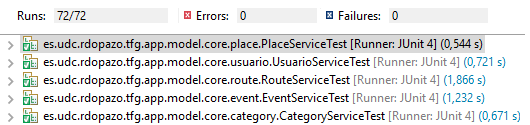
\includegraphics[
   keepaspectratio=true
]{./07_Pruebas/img/test2.png}}
\caption{Diagrama pruebas ejecutadas}
\end{figure}

Se han realizado un total de 72 pruebas sobre los diferentes casos de uso de cada servicio. En la figura siguiente, se podrá observar un ejemplo de cómo se han realizado estas pruebas.

\begin{figure}[H]
\centering
\fbox{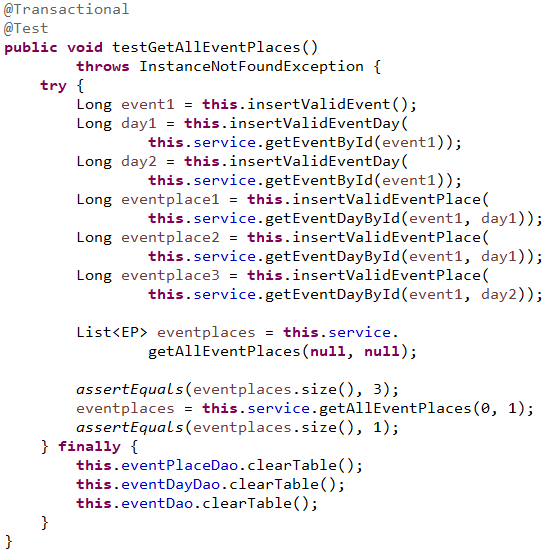
\includegraphics[
   keepaspectratio=true
]{./07_Pruebas/img/test1.png}}
\caption{Diagrama ejemplo - prueba JUnit}
\end{figure}


A mayores, también se comprobó la cobertura de las pruebas realizas sobre el código de la aplicación, obteniendo los siguiente resultados.

\begin{figure}[H]
\centering
\fbox{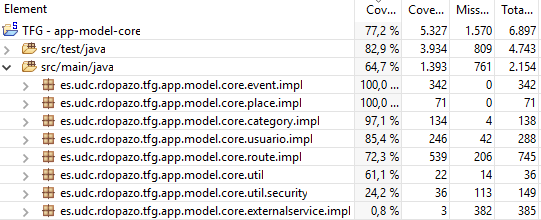
\includegraphics[
   keepaspectratio=true
]{./07_Pruebas/img/test3.png}}
\caption{Diagrama cobertura ejecución pruebas}
\end{figure}

Cabe destacar que los servicios externos no fueron incluidos en las pruebas automatizadas así como las clases del sub-paquete \textit{security}, y algunos casos de uso relacionados con usuarios y rutas que requieren una perspectiva global en la que se controle la autenciación de usuarios y el uso de los datos obtenidos de las fuentes externas.

A pesar de estas excepciones, las pruebas cubren más del 77\% de las líneas de código del módulo \textit{model-core}.


\section{Pruebas de sistema}
El objetivo de estas pruebas es comprobar el correcto funcionamiento del sistema software completo e integrado. Para ello, se realizaron el mayor número de pruebas posibles, 

Se realizaron pruebas de sistema para cada uno de los grandes bloques de la aplicación global. Por una parte, se realizaron pruebas sobre el servicio REST mediante el uso de herramientas de API testing, como  es Postman. Posteriormente, se probaron los dos clientes, web y móvil, independientemente, comprobándose el correcto funcionamiento de cada uno de ellos.

